\documentclass[11pt,a4paper]{article}
\usepackage[utf8]{inputenc}
\usepackage{graphicx}
\usepackage{geometry}
\usepackage{listings}
\usepackage{xcolor}
\usepackage{fancyhdr}
\usepackage{titlesec}
\usepackage{url}
\usepackage{float}

% Page setup
\geometry{left=2cm,right=2cm,top=2.5cm,bottom=2.5cm}
\pagestyle{fancy}
\fancyhf{}
\rhead{FIT5032 Assessed Lab 8}
\lhead{Firestore Integration}
\cfoot{\thepage}

% Code listing style
\lstset{
    basicstyle=\footnotesize\ttfamily,
    breaklines=true,
    frame=single,
    numbers=left,
    numberstyle=\tiny,
    showstringspaces=false,
    commentstyle=\color{gray},
    keywordstyle=\color{blue},
    stringstyle=\color{red}
}

\title{\textbf{FIT5032 Assessed Lab 8 Submission\\Firestore Database Integration}}
\author{Student Name: [Du Daoan]\\Student ID: [35523166]}
\date{}

\begin{document}

\maketitle

% =============================================================================
% EFOLIO TASK 8.1 (PASS AND CREDIT LEVEL)
% =============================================================================

\section{EFOLIO TASK 8.1 - Basic Firestore Integration}

\subsection{Screenshot Set 1: Add Book Implementation}

\subsubsection{Browser View}
\begin{figure}[H]
    \centering
    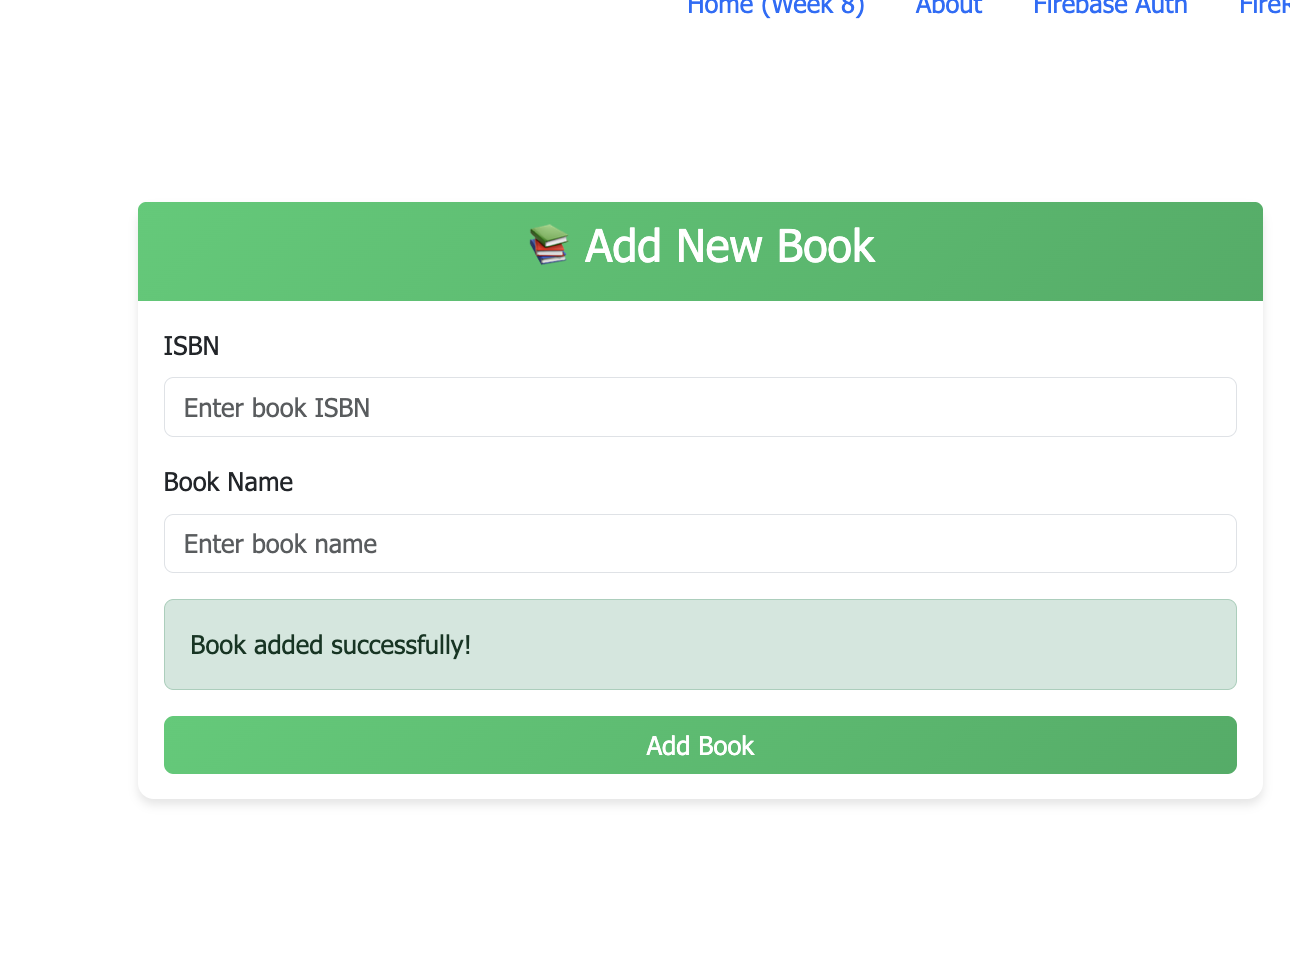
\includegraphics[width=0.9\textwidth]{add_book_browser.png}
    \caption{AddBookView.vue page showing the form and book list}
    \label{fig:add_book_browser}
\end{figure}

\textbf{Required:} Screenshot showing the AddBook page with form and book list components.

\subsubsection{Visual Studio Code Implementation}
% \begin{figure}[H]
%     \centering
%     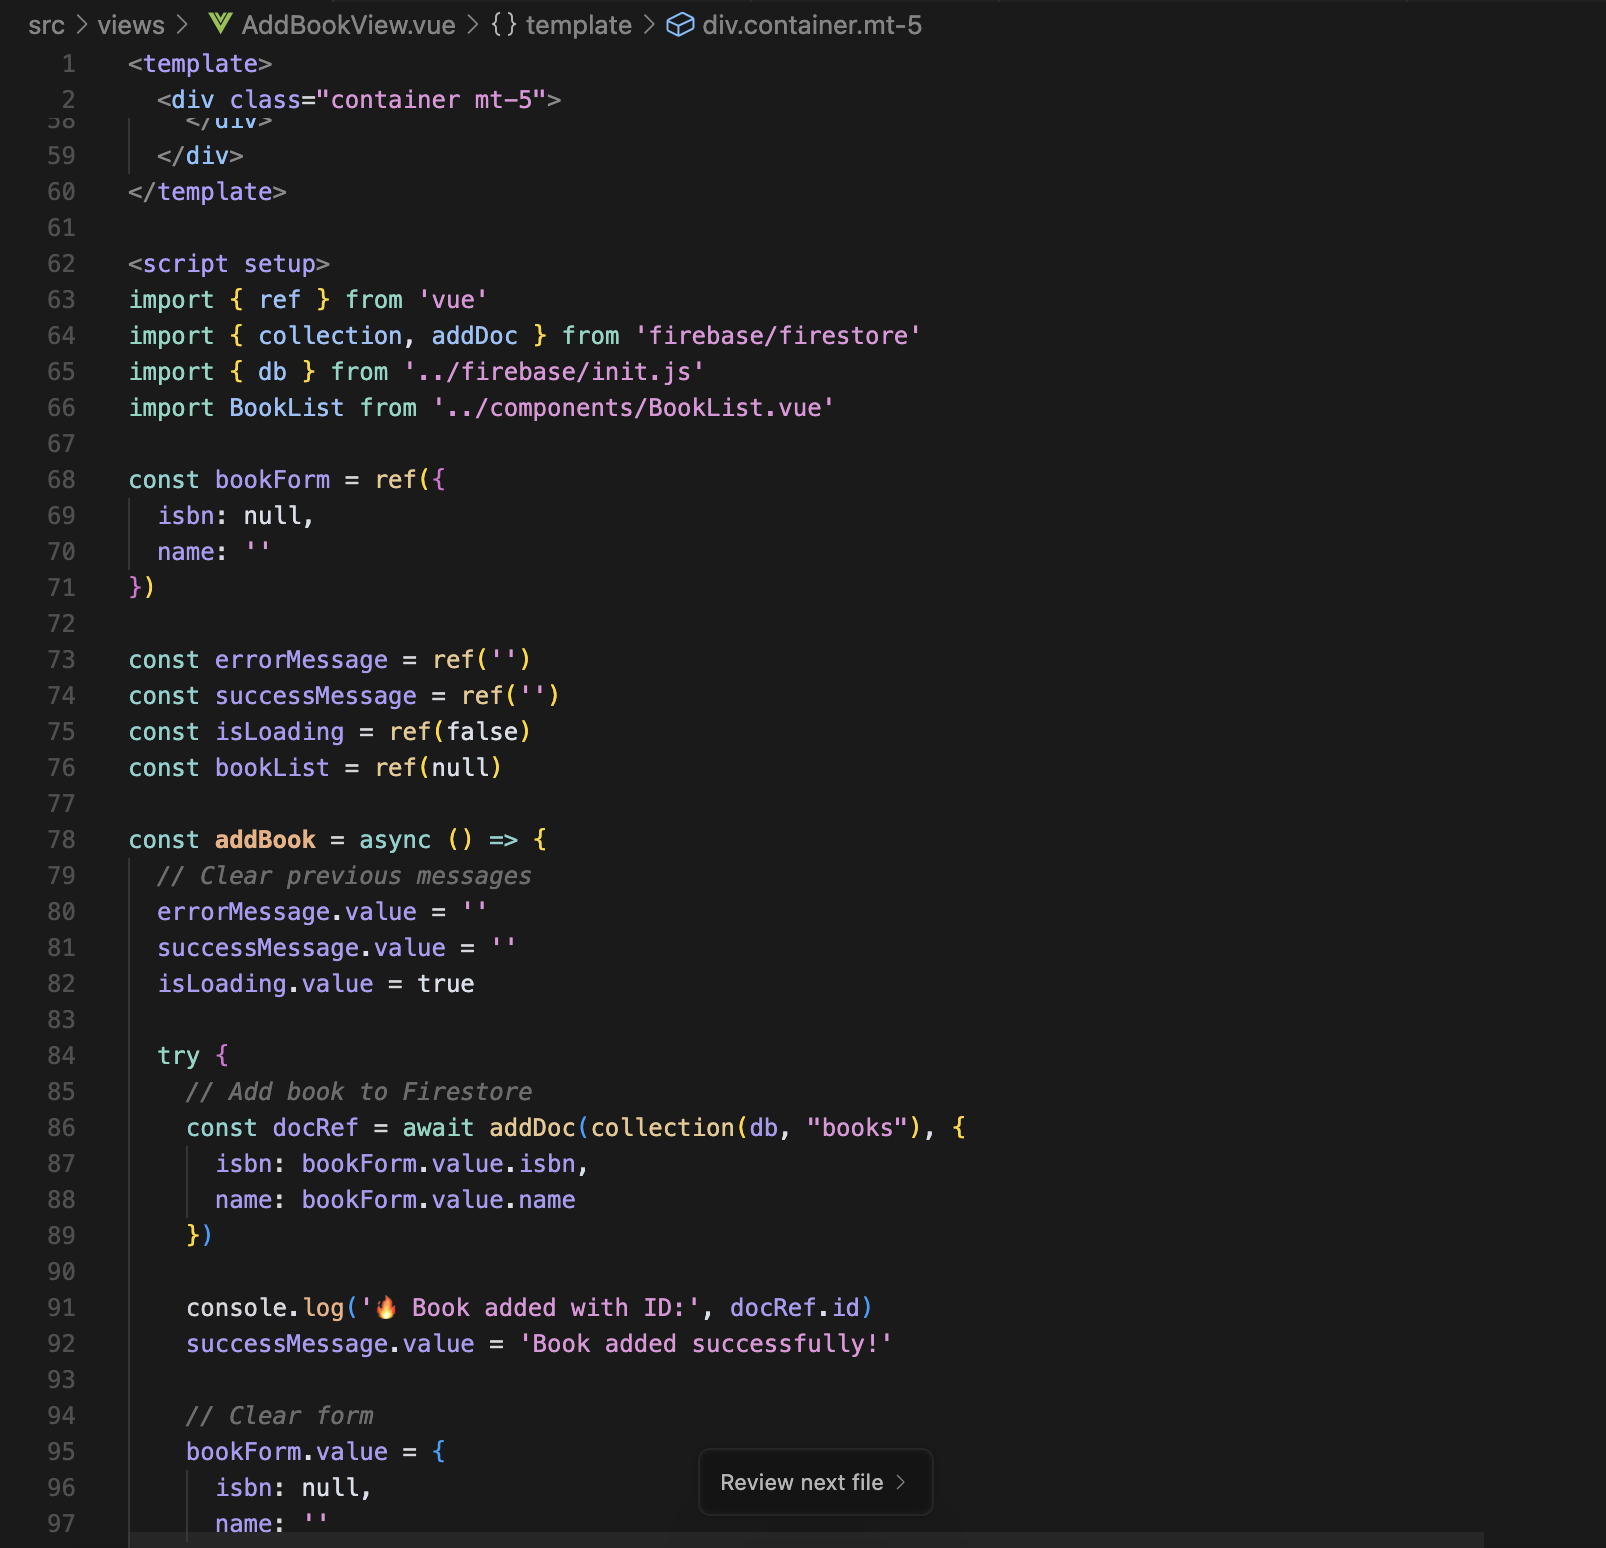
\includegraphics[width=0.9\textwidth]{add_book_vscode.png}
%     \caption{AddBookView.vue implementation in VS Code}
%     \label{fig:add_book_vscode}
% \end{figure}

\textbf{Required:} Screenshot showing the AddBookView.vue code implementation.

\subsection{Screenshot Set 2: Firestore Database}

 \begin{figure}[H]
    \centering
    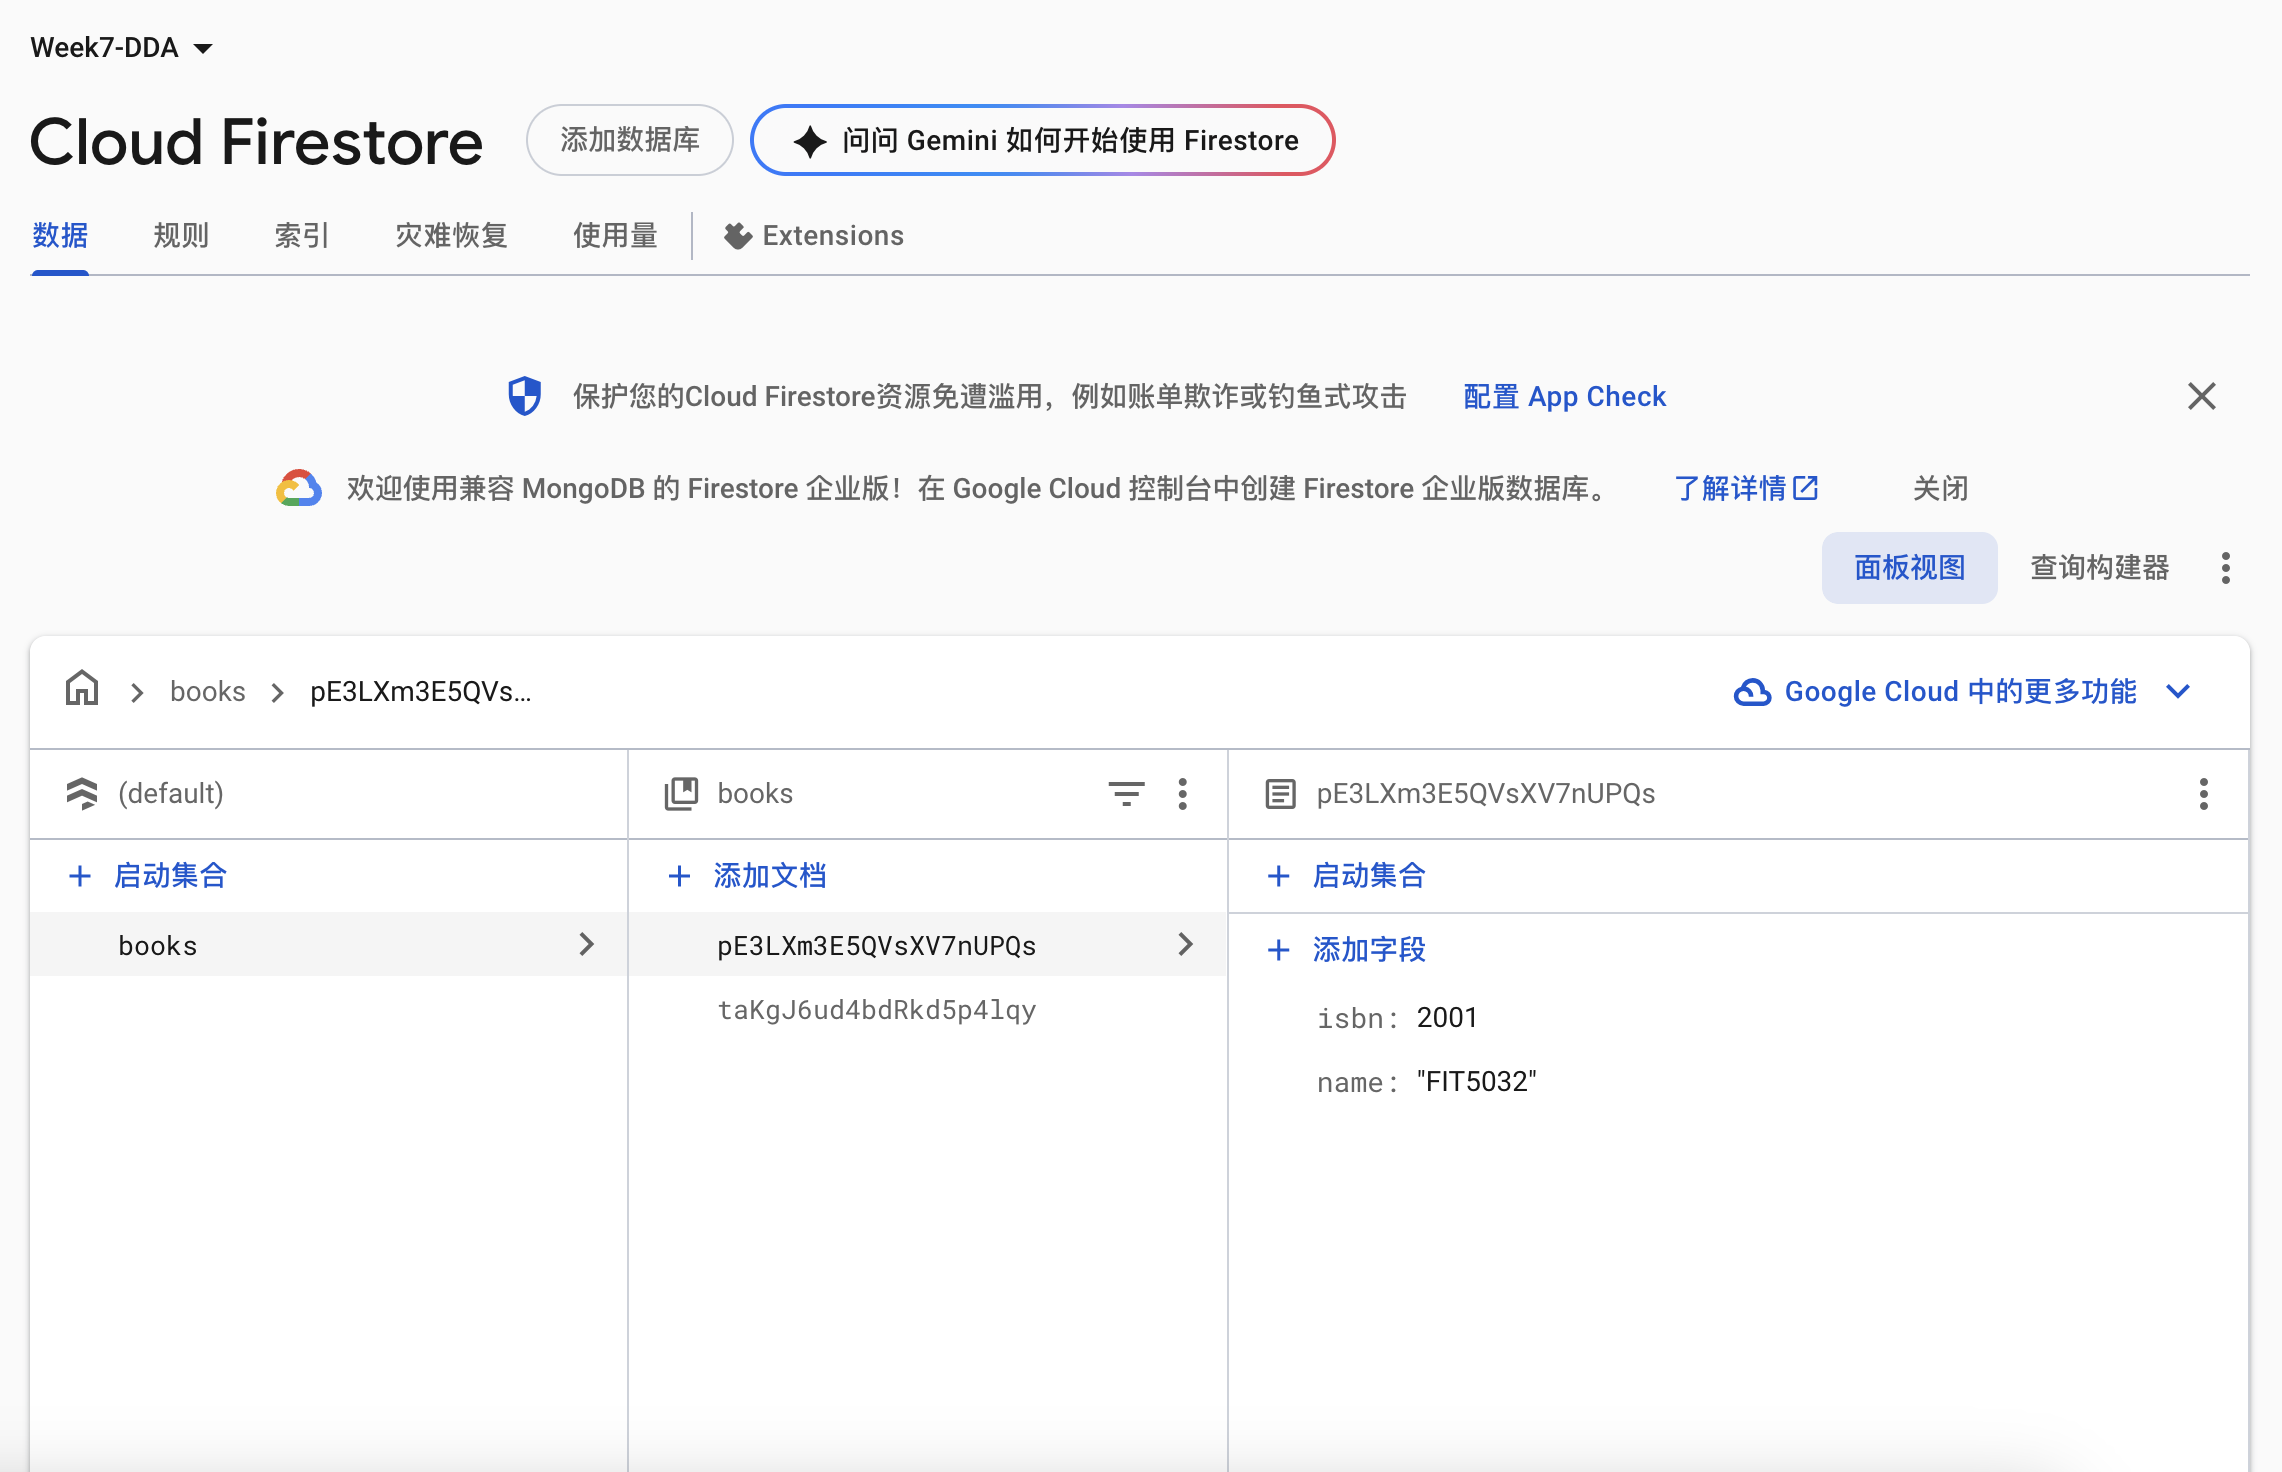
\includegraphics[width=0.9\textwidth]{firestore_data.png}
    \caption{Firestore console showing added book data}
    \label{fig:firestore_data}
\end{figure}

\textbf{Required:} Screenshot of Firestore console showing the books collection with added data.

\newpage

% =============================================================================
% EFOLIO TASK 8.2 (DISTINCTION AND HIGH DISTINCTION LEVEL)
% =============================================================================

\section{EFOLIO TASK 8.2 - Advanced Firestore Operations}

\subsection{Screenshot Set 1: Update and Delete Operations}

\subsubsection{Update Operation}
 \begin{figure}[H]
    \centering
    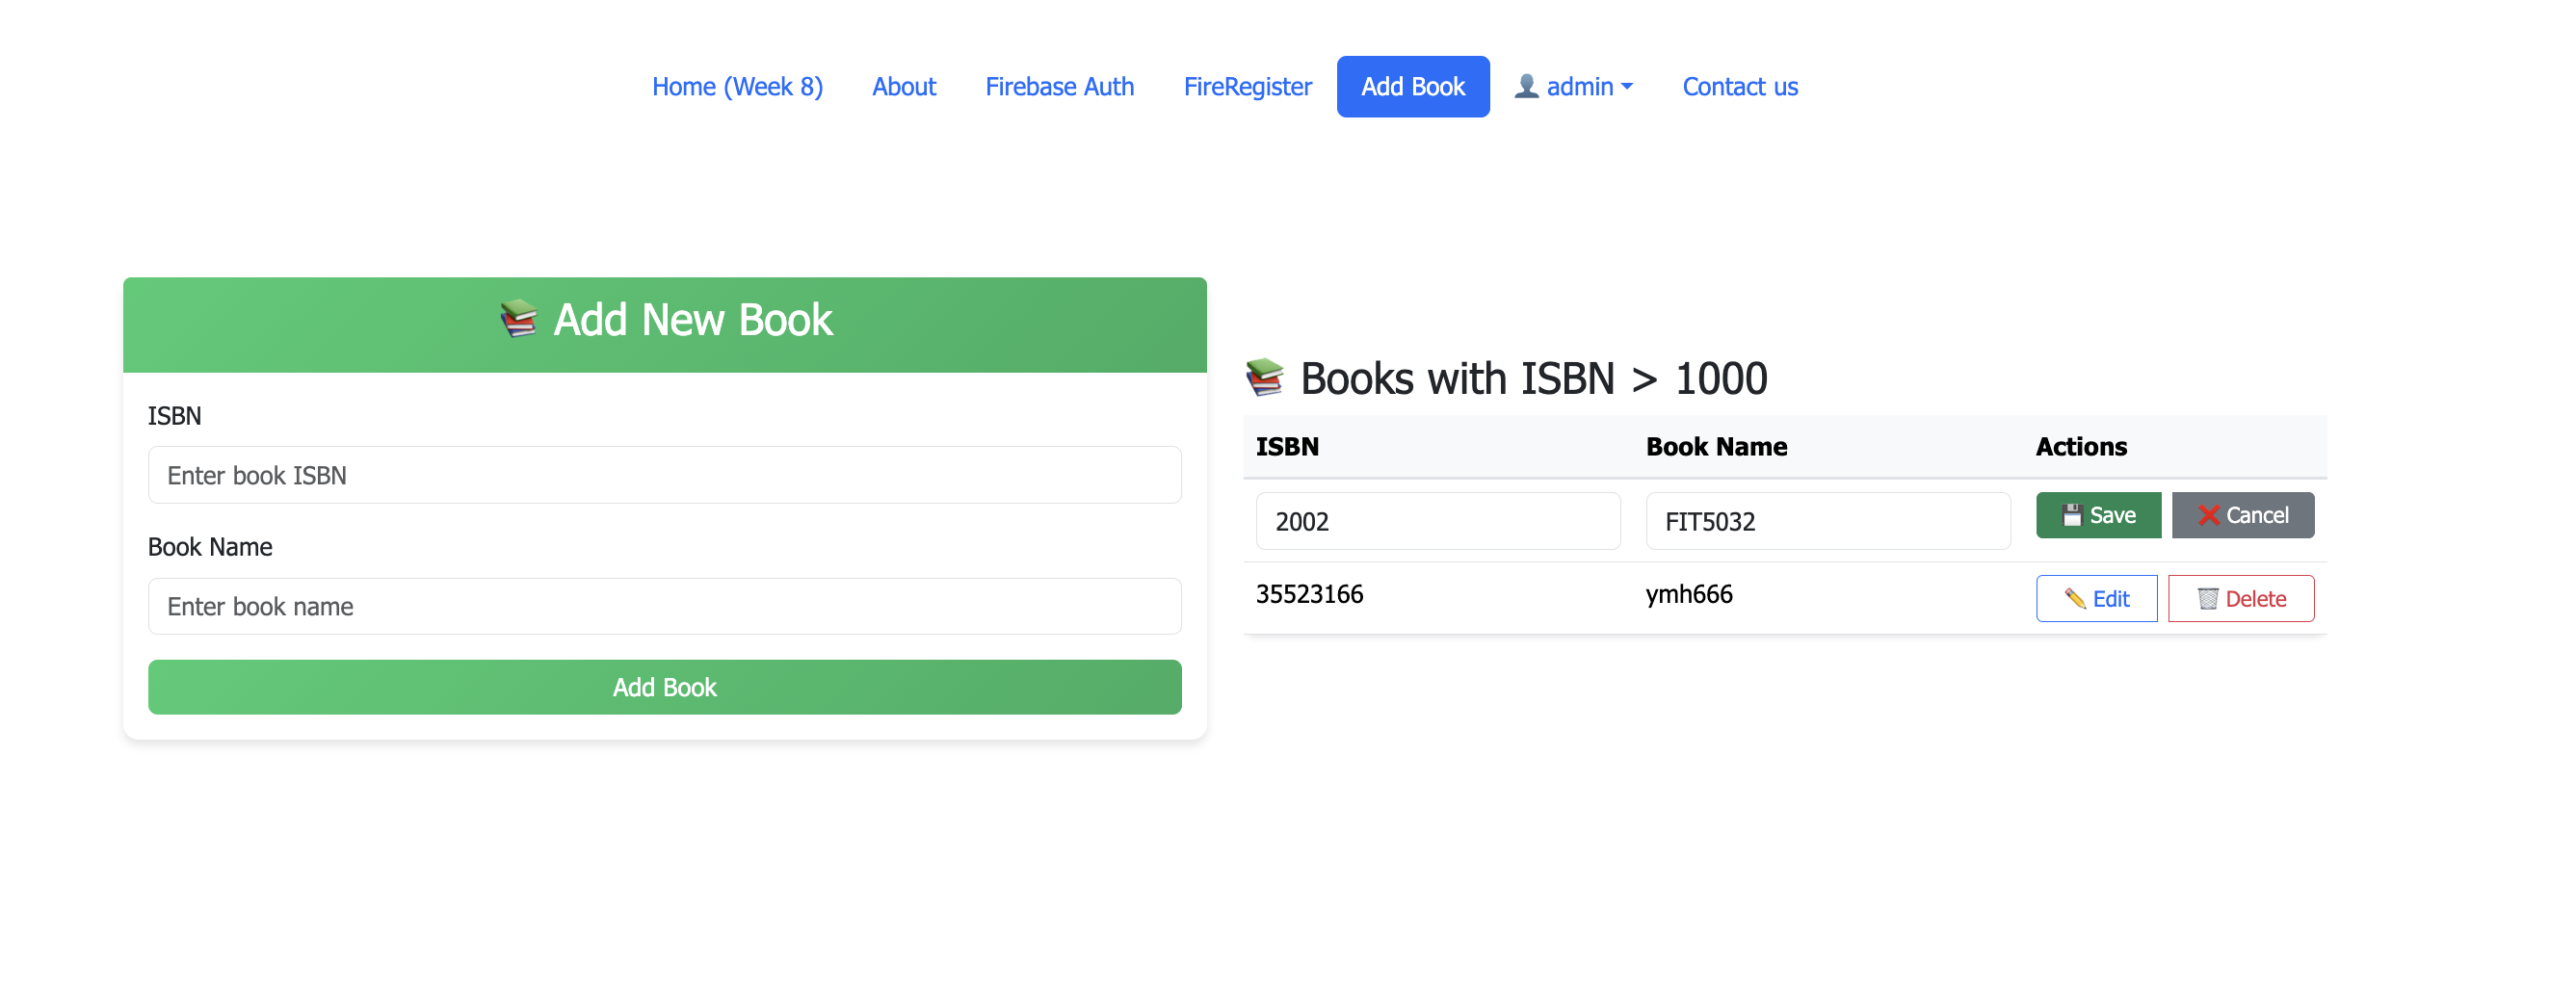
\includegraphics[width=0.9\textwidth]{update_book_browser.png}
    \caption{Book update functionality in browser}
    \label{fig:update_book_browser}
 \end{figure}

 \begin{figure}[H]
    \centering
    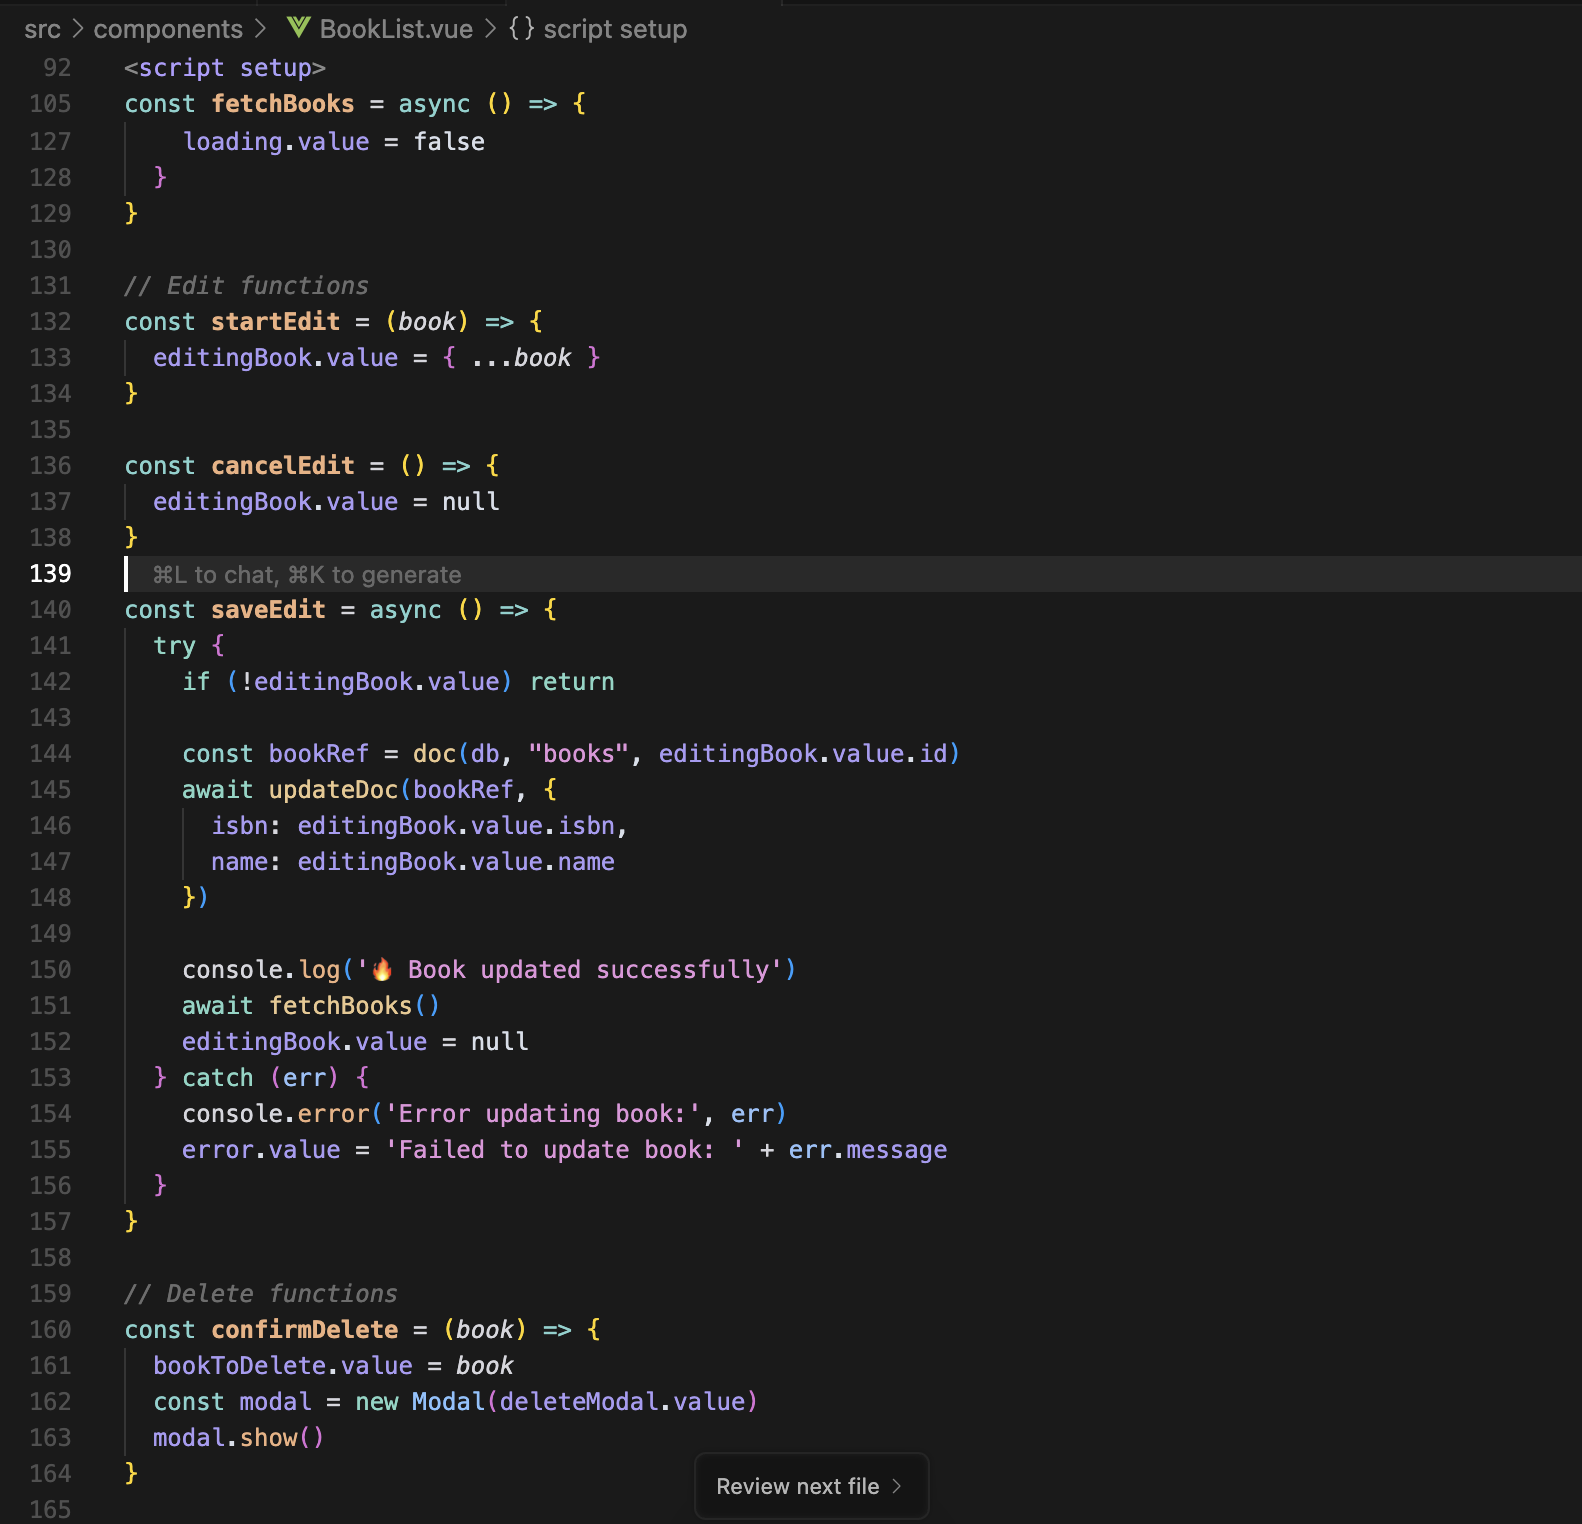
\includegraphics[width=0.9\textwidth]{update_book_code.png}
    \caption{Update implementation in VS Code}
    \label{fig:update_book_code}
 \end{figure}

\subsubsection{Delete Operation}
 \begin{figure}[H]
    \centering
    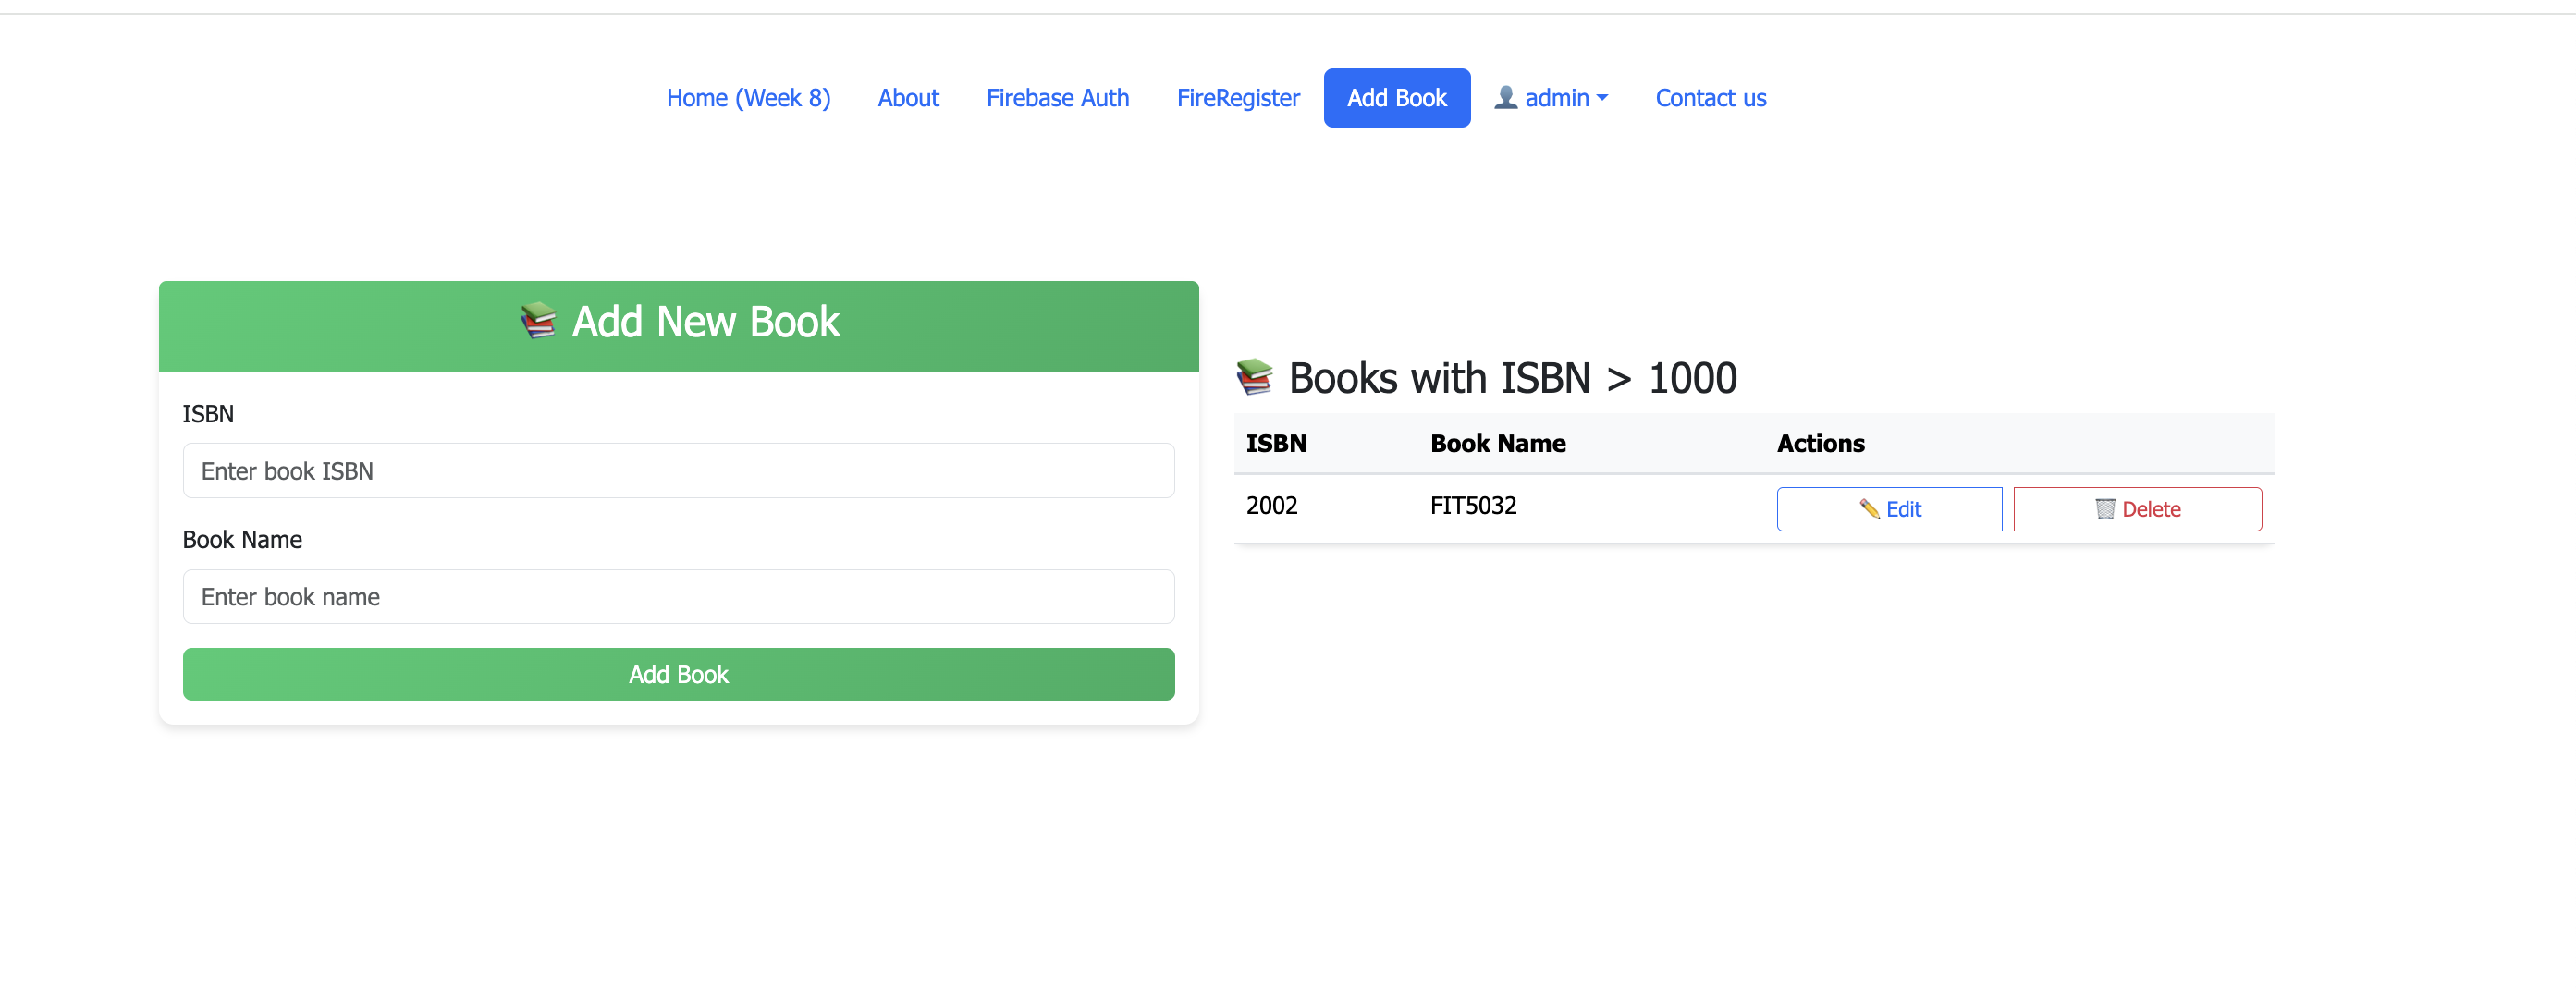
\includegraphics[width=0.9\textwidth]{delete_book_browser.png}
    \caption{Book deletion functionality in browser}
    \label{fig:delete_book_browser}
 \end{figure}

 \begin{figure}[H]
     \centering
     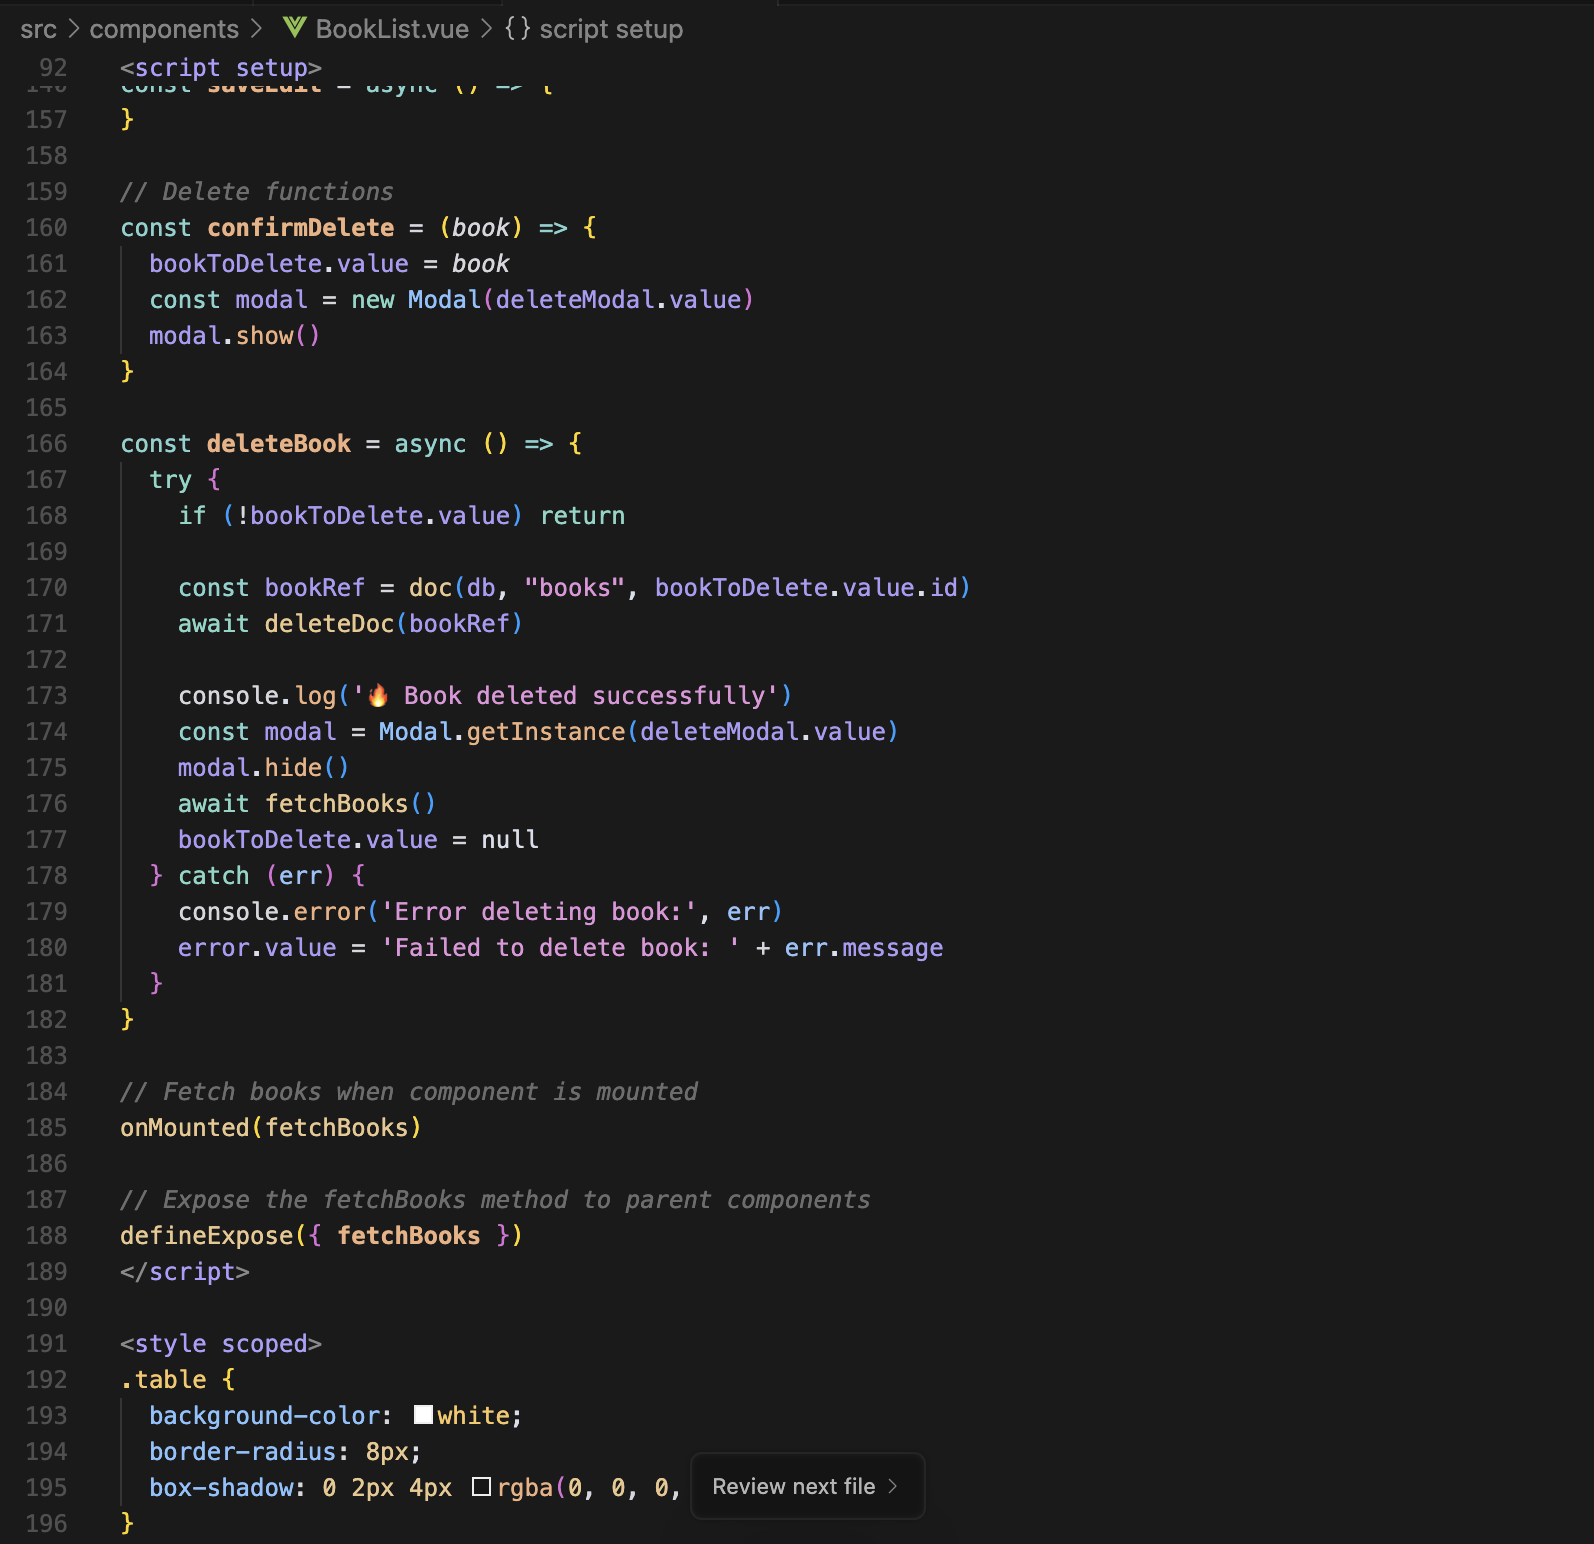
\includegraphics[width=0.9\textwidth]{delete_book_code.png}
     \caption{Delete implementation in VS Code}
     \label{fig:delete_book_code}
 \end{figure}

\subsection{Screenshot Set 2: Advanced Queries}

\subsubsection{Query Implementation}
 \begin{figure}[H]
     \centering
     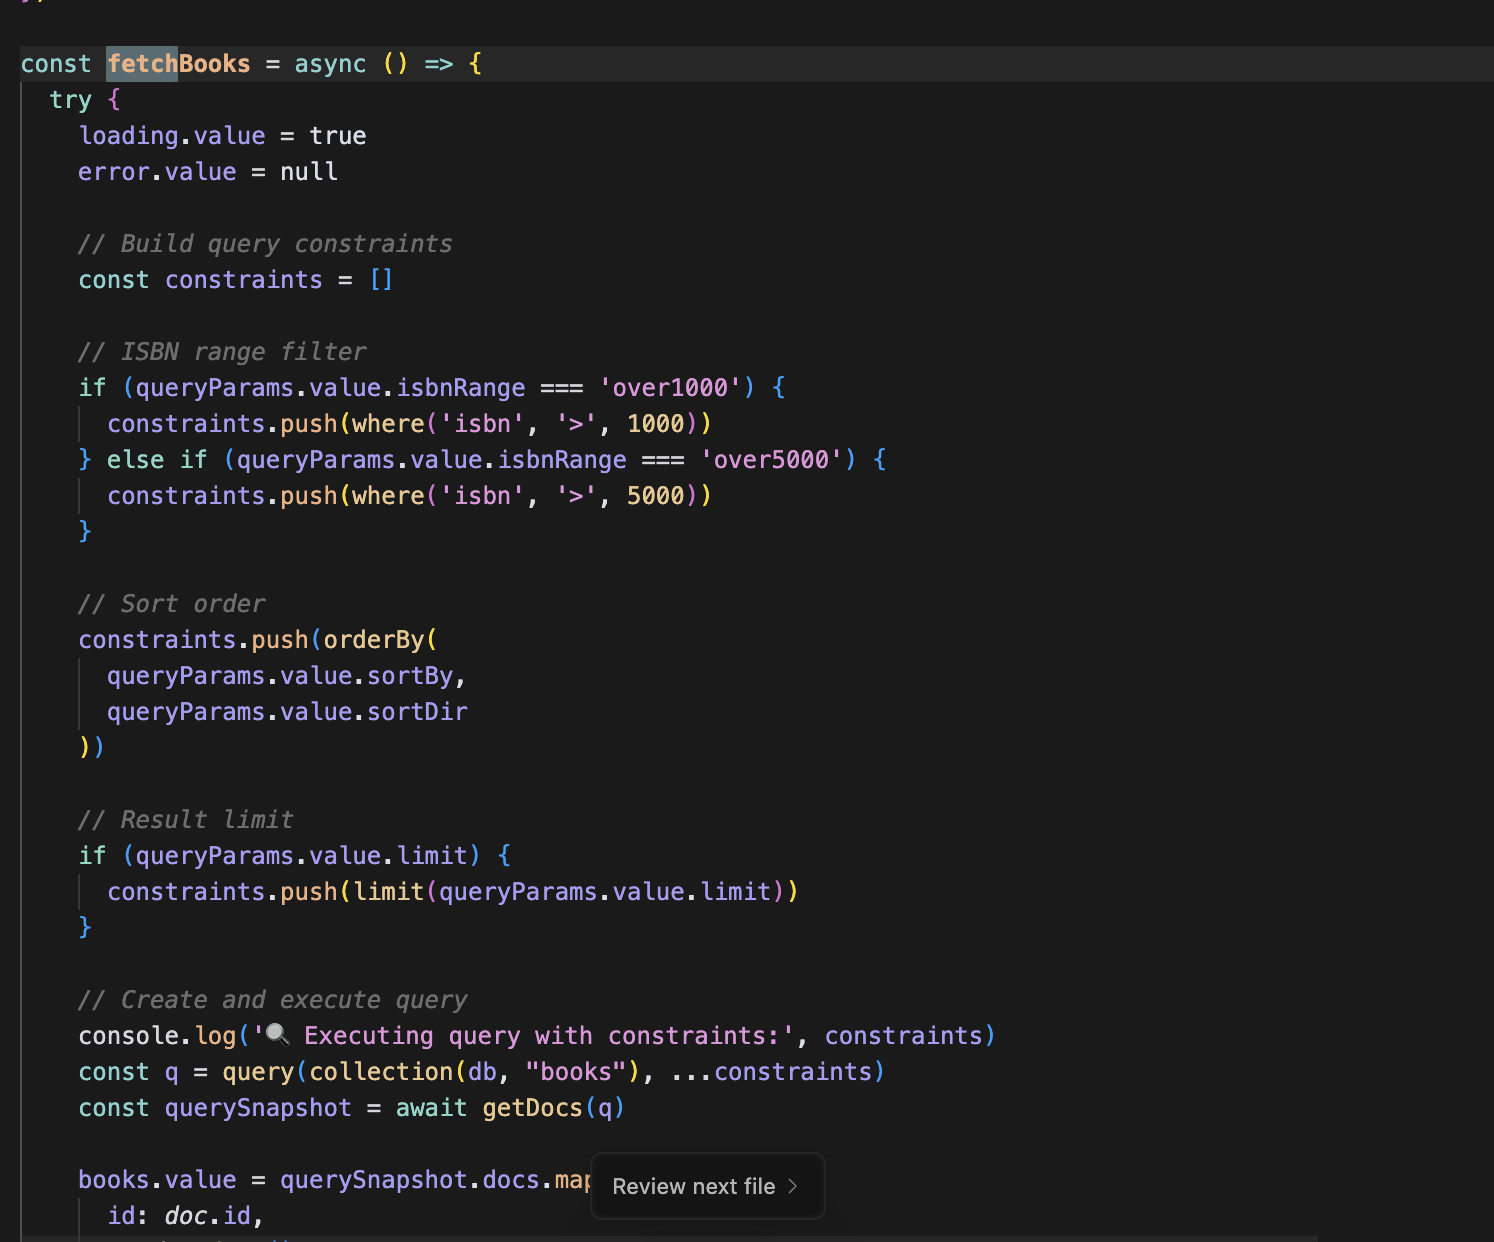
\includegraphics[width=0.9\textwidth]{query_implementation.png}
     \caption{Implementation of where, orderBy, and limit queries}
     \label{fig:query_implementation}
 \end{figure}

\subsubsection{Query Results}
 \begin{figure}[H]
     \centering
     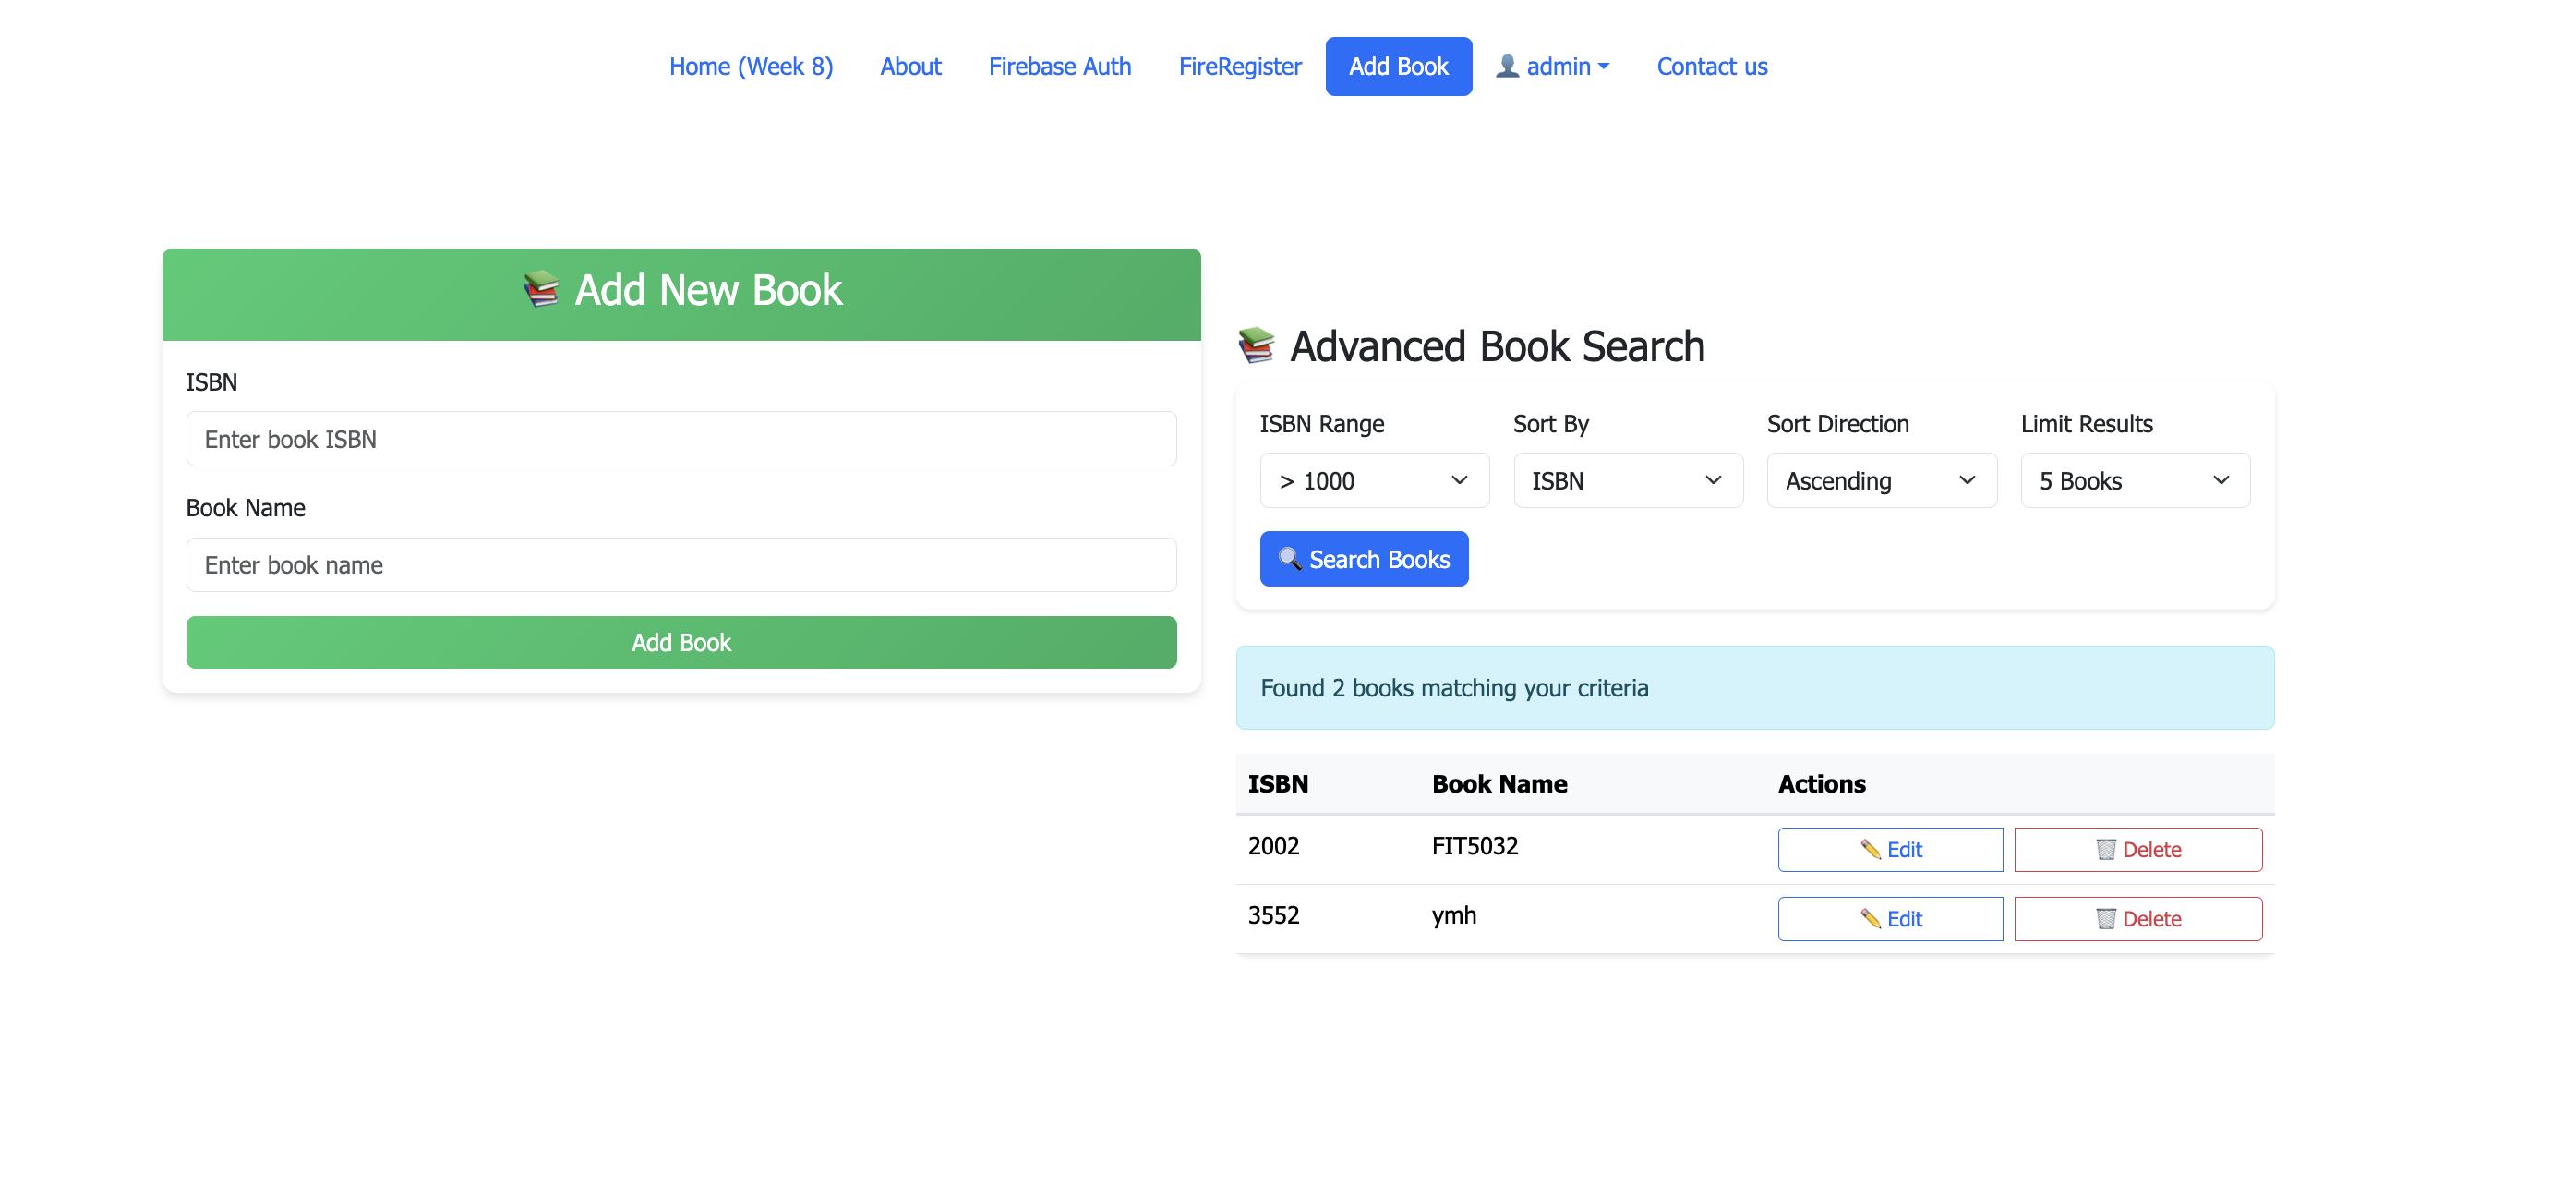
\includegraphics[width=0.9\textwidth]{query_results.png}
     \caption{Query results displayed in browser}
     \label{fig:query_results}
 \end{figure}

\section{Technical Achievement Summary}

This implementation demonstrates:
\begin{itemize}
    \item \textbf{Firestore Integration:} Complete setup with Vue.js
    \item \textbf{CRUD Operations:} Create, Read, Update, Delete functionality
    \item \textbf{Advanced Queries:} Using where, orderBy, and limit
    \item \textbf{Real-time Updates:} Automatic UI updates on data changes
    \item \textbf{Component Architecture:} Reusable BookList component
    \item \textbf{Form Validation:} Required fields and type checking
    \item \textbf{Error Handling:} Proper error messages and loading states
\end{itemize}

\end{document} 